% JUMP TO LINE 60, 73
\documentclass[preview, margin=0.6in]{standalone}
\usepackage[letterpaper,portrait,top=0.4in, left=0.6in, right=0.6in, bottom=1in]{geometry}

\usepackage{amsmath, amsfonts, amsthm, amssymb}
\usepackage{graphicx, float}
\usepackage{mathtools}
\usepackage{titlesec}
\usepackage{interval}
\usepackage{hyperref}
\usepackage{siunitx}
\usepackage{titling}
\usepackage{vwcol}
\usepackage{setspace}
\usepackage{empheq}
\usepackage{cancel}
\usepackage{esdiff}
\usepackage{multicol}
\usepackage{mdframed}
\usepackage{esdiff}
\usepackage{tikzsymbols}
\usepackage{multicol}
\usepackage{tikz}
\usepackage{varwidth}
\usepackage{pgfplots}
\pgfplotsset{compat=1.18}
\intervalconfig {
	soft open fences
}

\newcommand{\alignedintertext}[1]{%
  \noalign{%
    \vskip\belowdisplayshortskip
    \vtop{\hsize=\linewidth#1\par
    \expandafter}%
    \expandafter\prevdepth\the\prevdepth
  }%
}

\newtheorem{lemma}{Lemma}

\renewcommand{\qedsymbol}{\Smiley[1.3]}
\newcommand*{\problem}[1]{\section*{Problem #1}}
\newcommand*{\aps}{\section*{AP Corner}}
\newcommand*{\deriv}[1][x]{\ensuremath{\dfrac{\mathrm{d}}{\mathrm{d}#1}}}
\newcommand*{\floor}[1]{\ensuremath{\lfloor #1\rfloor}}
\newcommand*{\lheqzero}{\ensuremath{\underset{\text{L'H}}{\overset{\left[\frac00\right]}{=}}}}
\newcommand*{\lheqinfty}{\ensuremath{\underset{\text{L'H}}{\overset{\left[\frac{\infty}{\infty}\right]}{=}}}}

\DeclareMathOperator{\DNE}{DNE}
\DeclareMathOperator{\sgn}{sgn}

\DeclareMathOperator{\arccsc}{arccsc}
\DeclareMathOperator{\arcsec}{arcsec}
\DeclareMathOperator{\arccot}{arccot}

\setlength{\parindent}{0pt}

%opening
\title{\vspace*{-30pt}Problem Set \#6}
\author{Jayden Li}
\date{\today}

% \allowdisplaybreaks
\postdisplaypenalty=100000

\begin{document}
\setstretch{1.25}
\fontsize{12pt}{12pt}\selectfont
\setlength{\abovedisplayskip}{0pt}
\maketitle
\problem{1}
Completed last year.

\problem{2}
Completed last year or in class.

\problem{3}
\begin{itemize}
	\item[(a)]
		\begin{align*}
			\deriv\sqrt{x^2+1}+C
			&=\frac{2x}{2\sqrt{x^2+1}}
			=\frac{x}{\sqrt{x^2+1}}
		\end{align*}
	\item[(b)]
		\begin{align*}
			\deriv\left[x\sin x+\cos x+C\right]
			&=\sin x+x\cos x-\sin x
			=x\cos x
		\end{align*}
	\item[(c)]
		\begin{align*}
		   \deriv[x]\left[\sin x-\frac13\sin^3x+C\right] 
		   &=\cos x-\frac13\cdot3\sin^2x\cos x
		   =\cos x-\left(1-\cos^2x\right)\cos x \\ 
		   &=\cos x-\left(\cos x-\cos^3x\right)
		   =\cos x-\cos x+\cos^3x
		   =\cos^3x
		\end{align*}
	\item[(d)]
		\begin{align*}
		    \deriv[x]\left[\frac{2}{3b^2}(bx-2a)\sqrt{a+bx}+C\right]
			&=\frac{2}{3b^2}\left(b \sqrt{a+bx}+(bx-2a)\cdot \frac{b}{2 \sqrt{a+bx}}\right) \\
			&=\frac{2}{3b^2}\left(\frac{2b(a+bx)}{2\sqrt{a+bx}}+\frac{b(bx-2a)}{2 \sqrt{a+bx}}\right) \\
			&=\frac{2}{3b^2}\cdot \frac{2ab+2b^2x+b^2x-2ab}{2 \sqrt{a+bx}} \\
			&=\frac{3b^2x}{3b^2 \sqrt{a+bx}}
			=\frac{x}{\sqrt{a+bx}}
		\end{align*}
\end{itemize}

\problem{4}
\begin{itemize}
	\item[(a)] Done in class.
	\item[(b)]
		\begin{align*}
		    \int\left(\sqrt{x^3}+\sqrt[3]{x^2}\right)\mathrm{d}x
			&=\frac{x^{\frac{4}{3}}}{\frac{4}{3}}+\frac{x^{\frac{5}{3}}}{\frac{5}{3}}+C 
			=\frac{3\sqrt[3]{x^4}}{4}+\frac{3\sqrt[3]{x^5}}{5}+C
		\end{align*}
	\item[(c)]
		\begin{align*}
			\int \left(1-t\right)\left(2+t^2\right)\,\mathrm{d}t
			&=\int\left(2+t^2-2t-t^3\right)\mathrm{d}t
			=2t+\frac{t^3}{3}-t^2-\frac{t^4}{4}+C
		\end{align*}
	\item[(d)]
		\begin{align*}
		    \int v\cdot \left(v^2+2\right)^2\,\mathrm{d}v
			&=\int v\left(v^4+4v^2+4\right)\,\mathrm{d}v
			=\int\left(v^5+4v^3+4v\right)\mathrm{d}v \\ 
			&=\frac{v^6}{6}+\frac{4v^4}{4}+\frac{4v^2}{2}+C
			=\frac{v^6}{6}+v^4+2v^2+C
		\end{align*}
	\item[(e)]
		\begin{align*}
		    \int \frac{x^3-2 \sqrt{x}}{x}\,\mathrm{d}x
			&=\int\left(x^2-2x^{-\frac12}\right)\mathrm{d}x
			=\frac{x^3}{3}-\frac{2x^{\frac12}}{\frac12}+C
			=\frac{x^3}{3}-4 \sqrt{x}+C
		\end{align*}
	\item[(f)]
		\begin{align*}
		    \int\left(u^2+1+\frac{1}{u^2}\right)\mathrm{d}u
			&=\frac{u^3}{3}+u+\frac{u^{-1}}{-1}+C
			=\frac{u^3}{3}+u-\frac1u+C
		\end{align*}
	\item[(g)]
		\begin{align*}
		    \int\left(\theta-\csc\theta\cot\theta\right)\mathrm{d}\theta
			&=\int \theta\,\mathrm{d}\theta+\int\left(-\csc\theta\cot\theta\right)\,\mathrm{d}\theta
			=\frac{\theta^2}{2}+\csc\theta+C
		\end{align*}
	\item[(h)]
		\begin{align*}
		    \int \sec(t)(\sec t+\tan t)\,\mathrm{d}t
			&=\int\left(\sec^2t+\sec(t)\tan(t)\right)\mathrm{d}t
			=\tan t+\sec t+C
		\end{align*}
	\item[(i)]
		\begin{align*}
		    \int\left(1+\tan^2\alpha\right)\mathrm{d}\alpha
			&=\int\left(\frac{\cos^2\alpha}{\cos^2\alpha}+\frac{\sin^2\alpha}{\cos^2\alpha}\right)\mathrm{d}\alpha
			=\int \frac{1}{\cos^2\alpha}\,\mathrm{d}\alpha
			=\int \sec^2\alpha\,\mathrm{d}\alpha
			=\tan\alpha+C
		\end{align*}
	\item[(j)] Done in class.
	\item[(k)] Done in class.
	\item[(l)] Done in class.
\end{itemize}

\problem{5}
\begin{itemize}
	\begin{minipage}{0.49\linewidth}
		\item[(a)]
			\phantom{}
			\begin{center}
				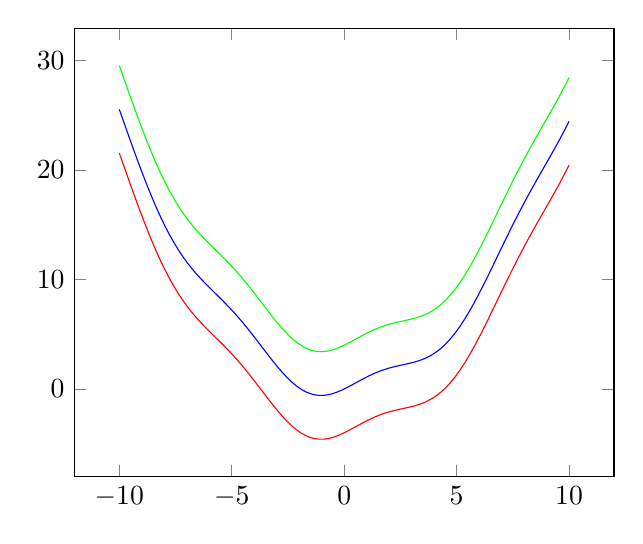
\begin{tikzpicture}
					\begin{axis}[domain=-10:10,legend pos=outer north east, samples=100]
					\addplot[red]{x^2/4 + sin(deg(x)) - 4};
					\addplot[blue]{x^2/4 + sin(deg(x))};
					\addplot[green]{x^2/4 + sin(deg(x)) + 4};
				\end{axis}
				\end{tikzpicture}
			\end{center}
	\end{minipage}\begin{minipage}{0.49\linewidth}
		\item[(b)]
			\phantom{}
			\begin{center}
				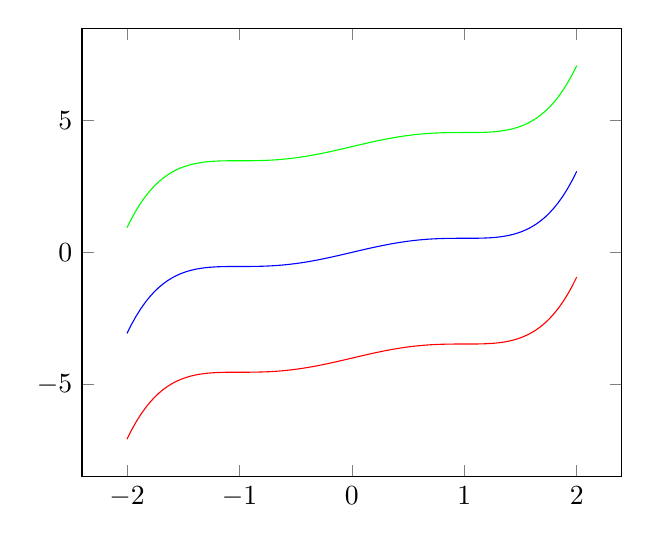
\begin{tikzpicture}
				\begin{axis}[domain=-2:2,legend pos=outer north east, samples=100]
					\addplot[red]{x-2*x^3/3+x^5/5 - 4};
					\addplot[blue]{x-2*x^3/3+x^5/5};
					\addplot[green]{x-2*x^3/3+x^5/5 + 4};
				\end{axis}
				\end{tikzpicture}
			\end{center}
	\end{minipage}
\end{itemize}

\problem{6}
\begin{itemize}
	\item[(a)]
		\begin{gather*}
			f(x)
			=\int\left(6 \sqrt{x}+5x^{3/2}\right)\mathrm{d}x
			=\frac{6x^{3/2}}{3/2}+\frac{5x^{5/2}}{5/2}+C
			=4 \sqrt{x^3}+2 \sqrt{x^5}+C \\
			f(1)=10 \implies 4+2+C=10 \implies C=4 \\
			\boxed{f(x)=4 \sqrt{x^3}+2 \sqrt{x^5}+4}
		\end{gather*}
	\item[(b)]
		\begin{gather*}
			f'(\theta)
			=\int\left(\sin\theta+\cos\theta\right)\mathrm{d}\theta
			=-\cos\theta+\sin\theta+C \\ 
			f'(0)=1 \implies -1+0+C=1 \implies C=2 \\
			f(\theta)
			=\int\left(-\cos\theta+\sin\theta+2\right)\mathrm{d}\theta
			=-\sin\theta-\cos\theta+2x+D \\
			f(0)=2 \implies 0-1+0+D=2 \implies D=3 \\ 
			\boxed{f(\theta)=-\sin\theta-\cos\theta+2x+3}
		\end{gather*}
\end{itemize}

\end{document}
